\documentclass[11pt, letterpaper]{memoir}
\usepackage{HomeworkStyle}
\geometry{margin=1in}



\begin{document}

	\begin{center}
		{\large Quiz 17.3 -- Reaction Mechanisms}
	\end{center}
	{\large Name: \rule[-1mm]{4in}{.1pt} 

\vspace{0.5em}\noindent
\begin{minipage}{0.35\linewidth}
\noindent\includegraphics[width=\linewidth]{MMKinetics}
\end{minipage}~~~
\begin{minipage}{0.65\linewidth}
\noindent On the figure at left, mark the values of $v_{max}$ and $K_M$ 

\vspace{6em}
~
\end{minipage}

\noindent Reaction rates for an enzyme-catalyzed reaction were recorded at different substrate concentrations. The data are tabulated below:

\noindent
\begin{tabular}{ccc}	
	Trial & Rate $\left(\nicefrac{M}{s}\right)$ & \ch{[S]_0} $\left(M\right)$ \\ \midrule \midrule
	1 &$2.7\times10^{-3}$&$0.0100$\\ \midrule
	2 &$3.5\times10^{-3}$&$0.0300$ \\ \midrule
\end{tabular}

\noindent Use these data to give $v_{max}$ and $K_M$ for the reaction

\vspace{10em}
\noindent For these trials, \ch{[E]_0}$=0.020M$. What is the catalytic efficiency, $\eta$, for the reaction?

\vspace{10em}
\noindent After an inhibitor is added, $v_{max}$ remains the same but $K_M$ is substantially greater. What type of inhibitor was added?

\vspace{8em}
\noindent
A fluorophore is known to have $k_F = 3.0\times10^{8}s^{-1}$, $k_{IC} = 1.0\times10^{8}s^{-1}$, and $k_{ISC} = 6.0\times10^{7}s^{-1}$

\noindent Give the observed fluorescence lifetime ($\tau$) and the quantum efficiency ($\phi_F$) for this fluorophore

\vspace{8em}
\noindent A quencher is then added to the solution and the quantum efficiency is monitored. Data for the trials are shown in the table below

\noindent
\begin{tabular}{cccc}	
	Trial & $\phi$ & $\frac{\phi_0}{\phi}$& \ch{[Q]} $\left(M\right)$ \\ \midrule \midrule
	1 &$0.513$&~\hspace{5em}~&$0.0010$\\ \midrule
	2 &$0.423$&&$0.0020$ \\ \midrule
\end{tabular}

\noindent Find the quenching rate constant $k_Q$ (with proper units)

\vspace{10em}
\noindent Assuming this quenching rate holds for auto-quenching, at what concentration of fluorophore will the quantum yield reach $10\%$ of its value in the dilute limit?

\vspace{4em}
\noindent
A pair of fluorophores is capable of F\"orster resonant energy transfer with $R_0=3.9nm$. These fluorophores are placed on two sites of a protein, and the energy transfer is observed to have $\eta_T=0.14$ ($14\%$ efficiency of energy transfer). What is the distance between the two sites on the protein?
\newpage
\pagestyle{empty}
\addtocounter{page}{-1}	
\section*{\emph{Your World}}
\paragraph{By Georgia Douglas Johnson}~
\begin{verse}
	Your world is as big as you make it.\\
	I know, for I used to abide\\
	In the narrowest nest in a corner,\\
	My wings pressing close to my side.
	
	But I sighted the distant horizon\\
	Where the skyline encircled the sea\\
	And I throbbed with a burning desire\\
	To travel this immensity.
	
	I battered the cordons around me\\
	And cradled my wings on the breeze,\\
	Then soared to the uttermost reaches\\
	With rapture, with power, with ease!
\end{verse}
\end{document}
